\section{Community subdivision}
Real-world network tend to be subdivided in many, smaller communities. This phenomenon is found in social networks \cite{barabasi283}, biological network \cite{barabasi288} and phone-call networks \cite{barabasi282}, and it has been of great interested for researchers since the early 2000s. One very good (and famous) example of the effect that the community subdivision can have on a network is the case known as \emph{Zachary's Karate Club} \cite{karateclub}. In this paper, the authors applied an autonomous community detection algorithm to the karate club participants' personal-interactions network which was able to predict the exact way in which the network fell apart after one major conflict struck the club.

This example illustrates how community detection can be a useful tool to quantify the robustness of a given network and to potentially predict its modes of failure under stress. In this chapter, I will briefly explain how communities can be defined and I will show how the Trainline network is subdivided.

\subsection{Defining communities}
Currently, there is not any widely-accepted definition of \emph{community}. Moreover, the mere existence of communities currently lacks any deep mathematical proofs and is based only upon empirical observations.  Barabasi \cite{barabasi} defines communities by using a series of hypotheses:
\begin{enumerate}
    \item Communities are structures uniquely encoded in a network's wiring diagram. The \emph{ground truth} of the community structure is to be discovered with algorithms.
    \item A community corresponds to a connected subgraph, whose connections are denser than with the rest of the network.
    \item Random networks do not have communities.
\end{enumerate}

Algorithms for community detection are constantly being developed \cite{communityDetection}; the main challenge for new algorithm is the difficulty in obtaining good results while maintaining a low computational complexity.
Given that the number of possible partition in a graph scales exponentially with its number of nodes \cite{barabasi}, a  simple brute-force approach would not work.

Currently, the best scaling algorithm is the Louvain method \cite{barabasi282}, which scales linearly with the number of links ($\mathcal O(L)$). There exist other algorithms that scale polinomially with the size of the network, up to the clique percolation algorithm \cite{cliquepercolation} which scales exponentially with the number of nodes ($\mathcal O(e^N)$). Ultimately, there does not exist a definitive \emph{best choice}; each algorithm has its own strength and weaknesses and should be used only within its intended use cases.

\subsection{Community detection results}
I have run a community detection algorithm on the Trainline network and the results are displayed in \autoref{fig:rainbow-plot}.
I have used the Mathematica function \verb|FindGraphCommunities| \cite{findgraphcommunities} with \verb|Methods->"Hierarchical"| settings. The official documentation does not state which exact algorithm the function implements, but it is most likely one of the hierarchical algorithms discussed in \cite{communityDetection}.

\begin{figure}
    \centering
    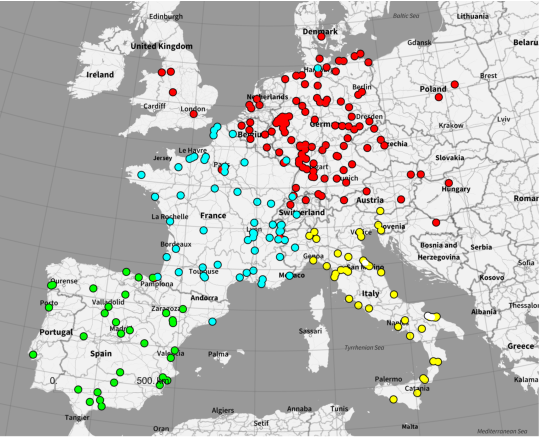
\includegraphics[width=1\linewidth]{report/assets/communitiesRainbow.pdf}
    \caption{Community structure of the Trainline network.
Four distinct communities are detected, roughly aligning with the geographic regions of Italy, France, Spain, and Germany. These regional clusters suggest that disruptions may cause localized isolation rather than complete network fragmentation.}
    \label{fig:rainbow-plot}
\end{figure}
Perhaps unsurprisingly, The algorithm managed to find four different communities which, for the most part, group the nodes which are situated in Italy, France, Spain and Germany. Given that, by definition, the link density is between community members is greater than with members of other communities, we can speculate that if the network were to face an attack, it would be less likely for a single community to immediately far apart, but more likely for different communities to remain isolated. 


\begin{figure}
    \centering
    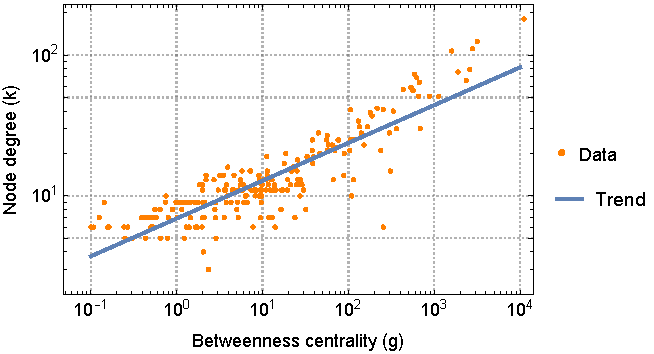
\includegraphics[width=1\linewidth]{report/assets/centralityDegreeCorrelation.pdf}
    \caption{Relationship between node degree and betweenness centrality.
    A positive correlation between the two is found, indicating that highly connected hubs also serve as primary paths in the network. This relationship shows how hubs are crucial in keeping the different communities connected together.}
    \label{fig:centrality-correlation}
\end{figure}
This is corroborated by the graph in \autoref{fig:centrality-correlation}, which shows that the degree of a certain node and its betweenness centrality are positively correlated. This, in turn, means that the more important a node is (i.e. the more links a certain city has), the higher is the number of shortest paths that pass through it. If an attack were to target the most important nodes first, it would make the travel time between nodes larger, up to infinity; if we assume that nodes in the same community are on average closer together, it is not unreasonable to assume that the shortest path between them will diverge slower than between nodes that are part of different communities.

The behavior of the network under an attack is discussed thoroughly in the next section.